% JuliaCon proceedings template
\documentclass{juliacon}
\setcounter{page}{1}
\usepackage{hyperref}

\begin{document}

% **************GENERATED FILE, DO NOT EDIT**************

\title{ProtoSyn.jl: a novel platform for computational molecular manipulation and simulation with a focus on protein design}

\author[1]{José M. S. Pereira}
\author[1]{José R. B. Gomes}
\author[1]{Sérgio M. Santos}
\affil[1]{Dep. Química \& CICECO, Universidade de Aveiro, Aveiro, Portugal}

\keywords{Julia, Protein Design, Molecular manipulation, Simulation}

\hypersetup{
pdftitle = {ProtoSyn.jl: a novel platform for computational molecular manipulation and simulation with a focus on protein design},
pdfsubject = {JuliaCon 2022 Proceedings},
pdfauthor = {José M. S. Pereira, José R. B. Gomes, Sérgio M. Santos},
pdfkeywords = {Julia, Protein Design, Molecular manipulation, Simulation},
}

\maketitle

\begin{abstract}

Modern protein design and drug discovery workflows harness the potential of computer simulations to prototype new effectors from the desired task, with applications in therapeutics, environment remediation and industrial settings, among others. In the recent decades, the field of computer sciences has seen tremendous growth, not only with the constant improvement in hardware power and availability, but also with the expansion of new techniques such as the usage of artificial intelligence, cloud \& high-performance computing, GPU acceleration and the introduction of modern programming languages. However, open-source scientific software targeted towards molecular simulation and protein design has lagged behind, mainly relying in outdated and poorly documented software, written in low-level programming languages and with decades of patches and hotfixes. ProtoSyn.jl, a novel platform for computational molecular manipulation and simulation, aims to offer an improved user experience. Written in Julia, a modern high-level scripting language, ProtoSyn.jl is fast, modular and includes a complete and comprehensive documentation manual with examples and use cases. Harnessing the power of open-source software, ProtoSyn.jl has the potential to modernize the way the scientific community uses simulation tools, bridging the gap between computational and experimental scientists. ProtoSyn.jl version 1.0, released July 2021, can be accessed at \href{https://github.com/sergio-santos-group/ProtoSyn.jl}{https://github.com/sergio-santos-group/ProtoSyn.jl}

\end{abstract}

\section{Introduction}

Traditionally, the goal of protein design and drug discovery was mainly pursued via experimental directed evolution or blind search \cite{Arnold1998, Jackel2008}. Such processes are lengthy and expensive, and often yield poor results. With the advent of modern computers, simulations and \emph{in silico} prototyping took precedence, quickly gaining traction as powerful tools to lower development times and costs, while increasing the accuracy of experimental efforts \cite{Huang2016}. In fact, over the last 20 years, the number of published papers in the computational chemistry field increased over 5-fold (measured by searching for the “computational chemistry” keywork in ScienceDirect).\vspace{5mm}

On the scope of protein design (and protein folding prediction), computer aided approaches have steadily increased in both complexity and accuracy, in great part due to the hegemony of the Rosetta software \cite{Pereira2021}. In 1999, Simons \emph{et al.}, from the Baker group, presented the first examples of homology-based methods for protein folding prediction, resulting in the release of the first version of Rosetta, written in Fortran \cite{Simons1999}. This early version of Rosetta was used to publish Top7, the first protein design of a novel topology \cite{Kuhlman2003}. This software was later translated into C++, in 2006, and wrapped multiple times in other languages, exposing some of the core functionalities, such as in Python, with Pyrosetta, in 2009 \cite{Chaudhury2010}. Over the last decade, the Rosetta family of scripts and software programs grew to include a large number of applications and scientific scopes (from ab initio modelling to NMR structure prediction) \cite{Leman2020}. Recently, and following incredible the work of AlphaFold, in CASP 13 \cite{Senior2020}, and AlphaFold2 in CASP 14 \cite{Tunyasuvunakool2021, Jumper2021}, the trRosetta application was published, using neural networks to predict protein structures \cite{Yang2020}.\vspace{5mm}

Other software solutions of notice include PyMOL and USCF ChimeraX \cite{Goddard2018}, albeit with a much narrower field of application (mainly focusing of molecular manipulation and visualization).\vspace{5mm}

It is possible to observe a common trend in the last 20 years of scientific software development for protein design: small scripts or software packages are developed and published for a specific task, often using Rosetta as the backend, and later bundled together. More often than not, computational design efforts make use of multiple tools, in multiple programming languages. This paradigm offers blatant disadvantages, such as the need for file type parsing scripts, non-existent or improper documentation, performance loss due to data sharing via the file system and the incapacitation of most users to add code modifications due to the usage of legacy or low-level programming languages (such as Fortran or C++, respectively). This, unsurprisingly, offer a massive resistance to adoption of unified workflows and posts a large entry barrier to non-specialized members of the scientific community \cite{Samish2017}. 
As such, and besides commonly known best practices and recommendations for writing good open source software \cite{Sarhan2019} (for example, using a code hosting and version control, namely GitHub), four additional requirements for a modern software solution tailored for protein design and molecular simulation can be defined:
\begin{itemize}
\item Performace – Protein design efforts often rely on algorithms with millions of calculation steps. For this reason, even a slight slow-down in performance can cost hours or days in simulation time. Languages such as Python and R are notoriously slow 17, while lower-level languages such as C or C++ offer much better performance at the expense of readability and an out-of-the-box experience. This is known as the “two-language problem” and arises from the need to have the core code in a low-level language and user interfaces in a higher-level language. A modern solution should avoid the two-language problem while maintaining the highest possible performance.\vspace{5mm}

\item Modular – A modular solution allows versatility without increasing code entropy: users should be able to add new functionalities as modules, making use of existing structures, in the same programming language and following the same general guidelines. This removes the need for data sharing via the file system and usage of file type parsing scripts, while allowing greater flexibility in customization of protocols and linkage between different algorithms.\vspace{5mm}

\item Well documented – Application-specific scripts are often developed and maintained “in-house”, frequently causing proper documentation to be overlooked. Code without appropriate documentation is often the root cause for costly and time-consuming errors, elevating the entry barrier to new users (especially non-specialized scientists). Good documentation should also include a properly maintained and curated list of examples and tutorials, as well as adequate unit testing, allowing for easier implementation of new features without the risk of code breaking changes.\vspace{5mm}

\item Scalable - In the past decade, a healthy number of new technologies have gained traction in the scope of computer sciences, such as the usage of machine learning and artificial intelligence models, GPU computing and cloud computing. A modern tool for protein design should be scalable in order to incorporate new emerging technologies as they become available in order to boost accuracy, security and performance.
\end{itemize}\vspace{5mm}

Despite the undeniable success of Rosetta, with its many iterations and years of development, the current patchwork of scripts and applications does not fully comply to these requirements: the Rosetta (C++) and PyRosetta (Python) still fall into the “two-language problem”; the Rosetta software is, for the most part, interfaced with by multiple individual applications, each for a particular use (although, as an alternative, the RosettaScripts allow users to create and modify protocols using an XML-based syntax, exposing some of the core functionality provided by Rosetta \cite{Fleishman2011}); the PyRosetta documentation is infamous for its lack of documentation and outdated examples; and finally, Rosetta does not directly benefit from modern GPU acceleration platforms. These shortcomings have been identified before, with interesting works such as the EGAD Library, but the proposed solutions failed to satisfy all of the above requirements, preventing mass adoption and eventually falling into discontinuity \cite{Chowdry2007}.\vspace{5mm}

In conclusion: there’s room for improvement.

\section{Developing a new tool}

ProtoSyn.jl (whose name is a mesh between the words “Prototyping” and “Synthetic”, and whose attempt at a logo is shown in Figure \ref{fig:ProtoSynArticle-IM1}) aims to be a novel platform for molecular manipulation and simulation, with an emphasis on protein design.

\begin{figure}[h]
\centering
\includegraphics[width=0.35\textwidth]{ProtoSynArticle-IM1}
\caption{\textbf{ProtoSyn.jl's logo.} Attempts to represent 3 $\alpha$-helix structures using Julia's logo colors.}
\label{fig:ProtoSynArticle-IM1}
\end{figure}

The development of ProtoSyn.jl started in early 2018, fueled by the need for a more open, well documented and flexible tool for protein design. Since the project’s inception, three key concepts guided the development process: ProtoSyn.jl should be an open-access project, built on modularity and aimed for non-expert usage. ProtoSyn.jl is completely written in Julia \cite{Bezanson2017, Bezanson2018}, a modern programming language specifically developed to solve the two-language problem. Besides taking advantage of the momentum being felt by the Julia environment, with a growing and active community, ProtoSyn.jl also benefits from many of the inherent features of this programming language, such as an easy scripting syntax (“Looks like Python …”) and good performance (“… runs like C!”), access to low-level methods (such as GPU and SIMD acceleration, using CUDA.jl and SIMD.jl), direct access to Python and C code calls (using PyCall.jl), native support for distributed computing and a growing number of useful packages (such as DataFrames.jl, Plots.jl and emerging solutions in the molecular simulation environment, such as Molly.jl and AtomsBase.jl). As such, ProtoSyn.jl’s current flagship features include:
\begin{itemize}
\item Complete molecular manipulation tools – One of the main objectives of ProtoSyn.jl is to offer a playground experience, where users can freely modify peptides and proteins. Sometimes, a hard part of the protocol is to simply introduce a quick change in the structure/sequence of the peptide. With this goal in mind, ProtoSyn.jl makes available methods in order to remove, add and mutate residues, remove and add sidechains, saturate structures with hydrogens, cut, copy and paste whole molecules or fragmented selections of chains, explore and create new rotamer libraries, freely rotate dihedrals, apply secondary structures, etc. Using ProtoSyn.jl’s Builder module adds the possibility to create and append peptides from scratch, using only the amino acids sequence, and adds the capacity to include non-canonical aminoacids (NCAA) and post-translational modifications (PTMs) such as methylation and phosphorylation.\vspace{5mm}
\item Complex simulation algorithms – In order to test new designs, ProtoSyn’s simulation environment uses Monte Carlo, iterated local search (ILS) and steepest descent algorithms, among others, to explore the conformational space. Besides the existing methods, users can also define custom drivers for the simulation.\vspace{5mm}
\item Fully customizable energy functions – As with any simulation package, a simulation’s accuracy is dictated by the energy function employed. Besides the default energy function provided by ProtoSyn.jl, a rich library of potentials \& machine learning models is made available for users to pick and choose from, creating a custom energy functions specifically suited to the task at hands. Some examples of available energy function terms include the usage of contact maps, the TorchANI machine learning potential, geometrical hydrogen bonds, steric clashes, coarse-grained solvation energy, Generalized-Born (GB) solvation potential, etc. Besides the existing components, users are encouraged to prototype and test new energy function components, with a complete guide in the documentation and auxiliary methods made available. Developing energy function components is inherently hard, thus providing a centralized space to carry out benchmarks, parameterization efforts and "plug-and-play" testing has been a major focus during development of ProtoSyn.jl.\vspace{5mm}
\item Rich selection syntax – An ample list of selection methods can be employed and combined with ease, using logical operators, to specify with precision the target atoms or regions for a particular modification, simulation or energy measurement.\vspace{5mm}
\item GPU and cloud computing – Making use of Julia’s inherent characteristics, ProtoSyn.jl includes native support for GPU acceleration of most heavy calculations. Including the Distributed.jl package extends the usage of ProtoSyn to multiple threads (and even multiple machines), further accelerating the simulation of multiple replicas simultaneously. This paradigm can also be applied in dedicated HPC contexts, easily incorporating ProtoSyn.jl in commonly used cloud computing platforms.\vspace{5mm}
\end{itemize}\vspace{5mm}

In short: ProtoSyn intends to be a playground for prototyping new designs and ideas, enhancing the early stages of new protocols and projects by quickly deploying fast, scalable and accurate simulations of the mutation, interaction of modification of interest.

\section{Under the hood}

Following the established practice, the main data structure in ProtoSyn.jl is called a Pose. In ProtoSyn.jl, this is a complete description of a molecular system, incorporating both a directed Graph (this defines the nature of the particles in the system, as well as the interactions between each other) and a State (defining the position of the particles and the energy landscape of the system), as schematically described in Figure \ref{fig:ProtoSynArticle-IM2}.

\begin{figure}[h]
\centering
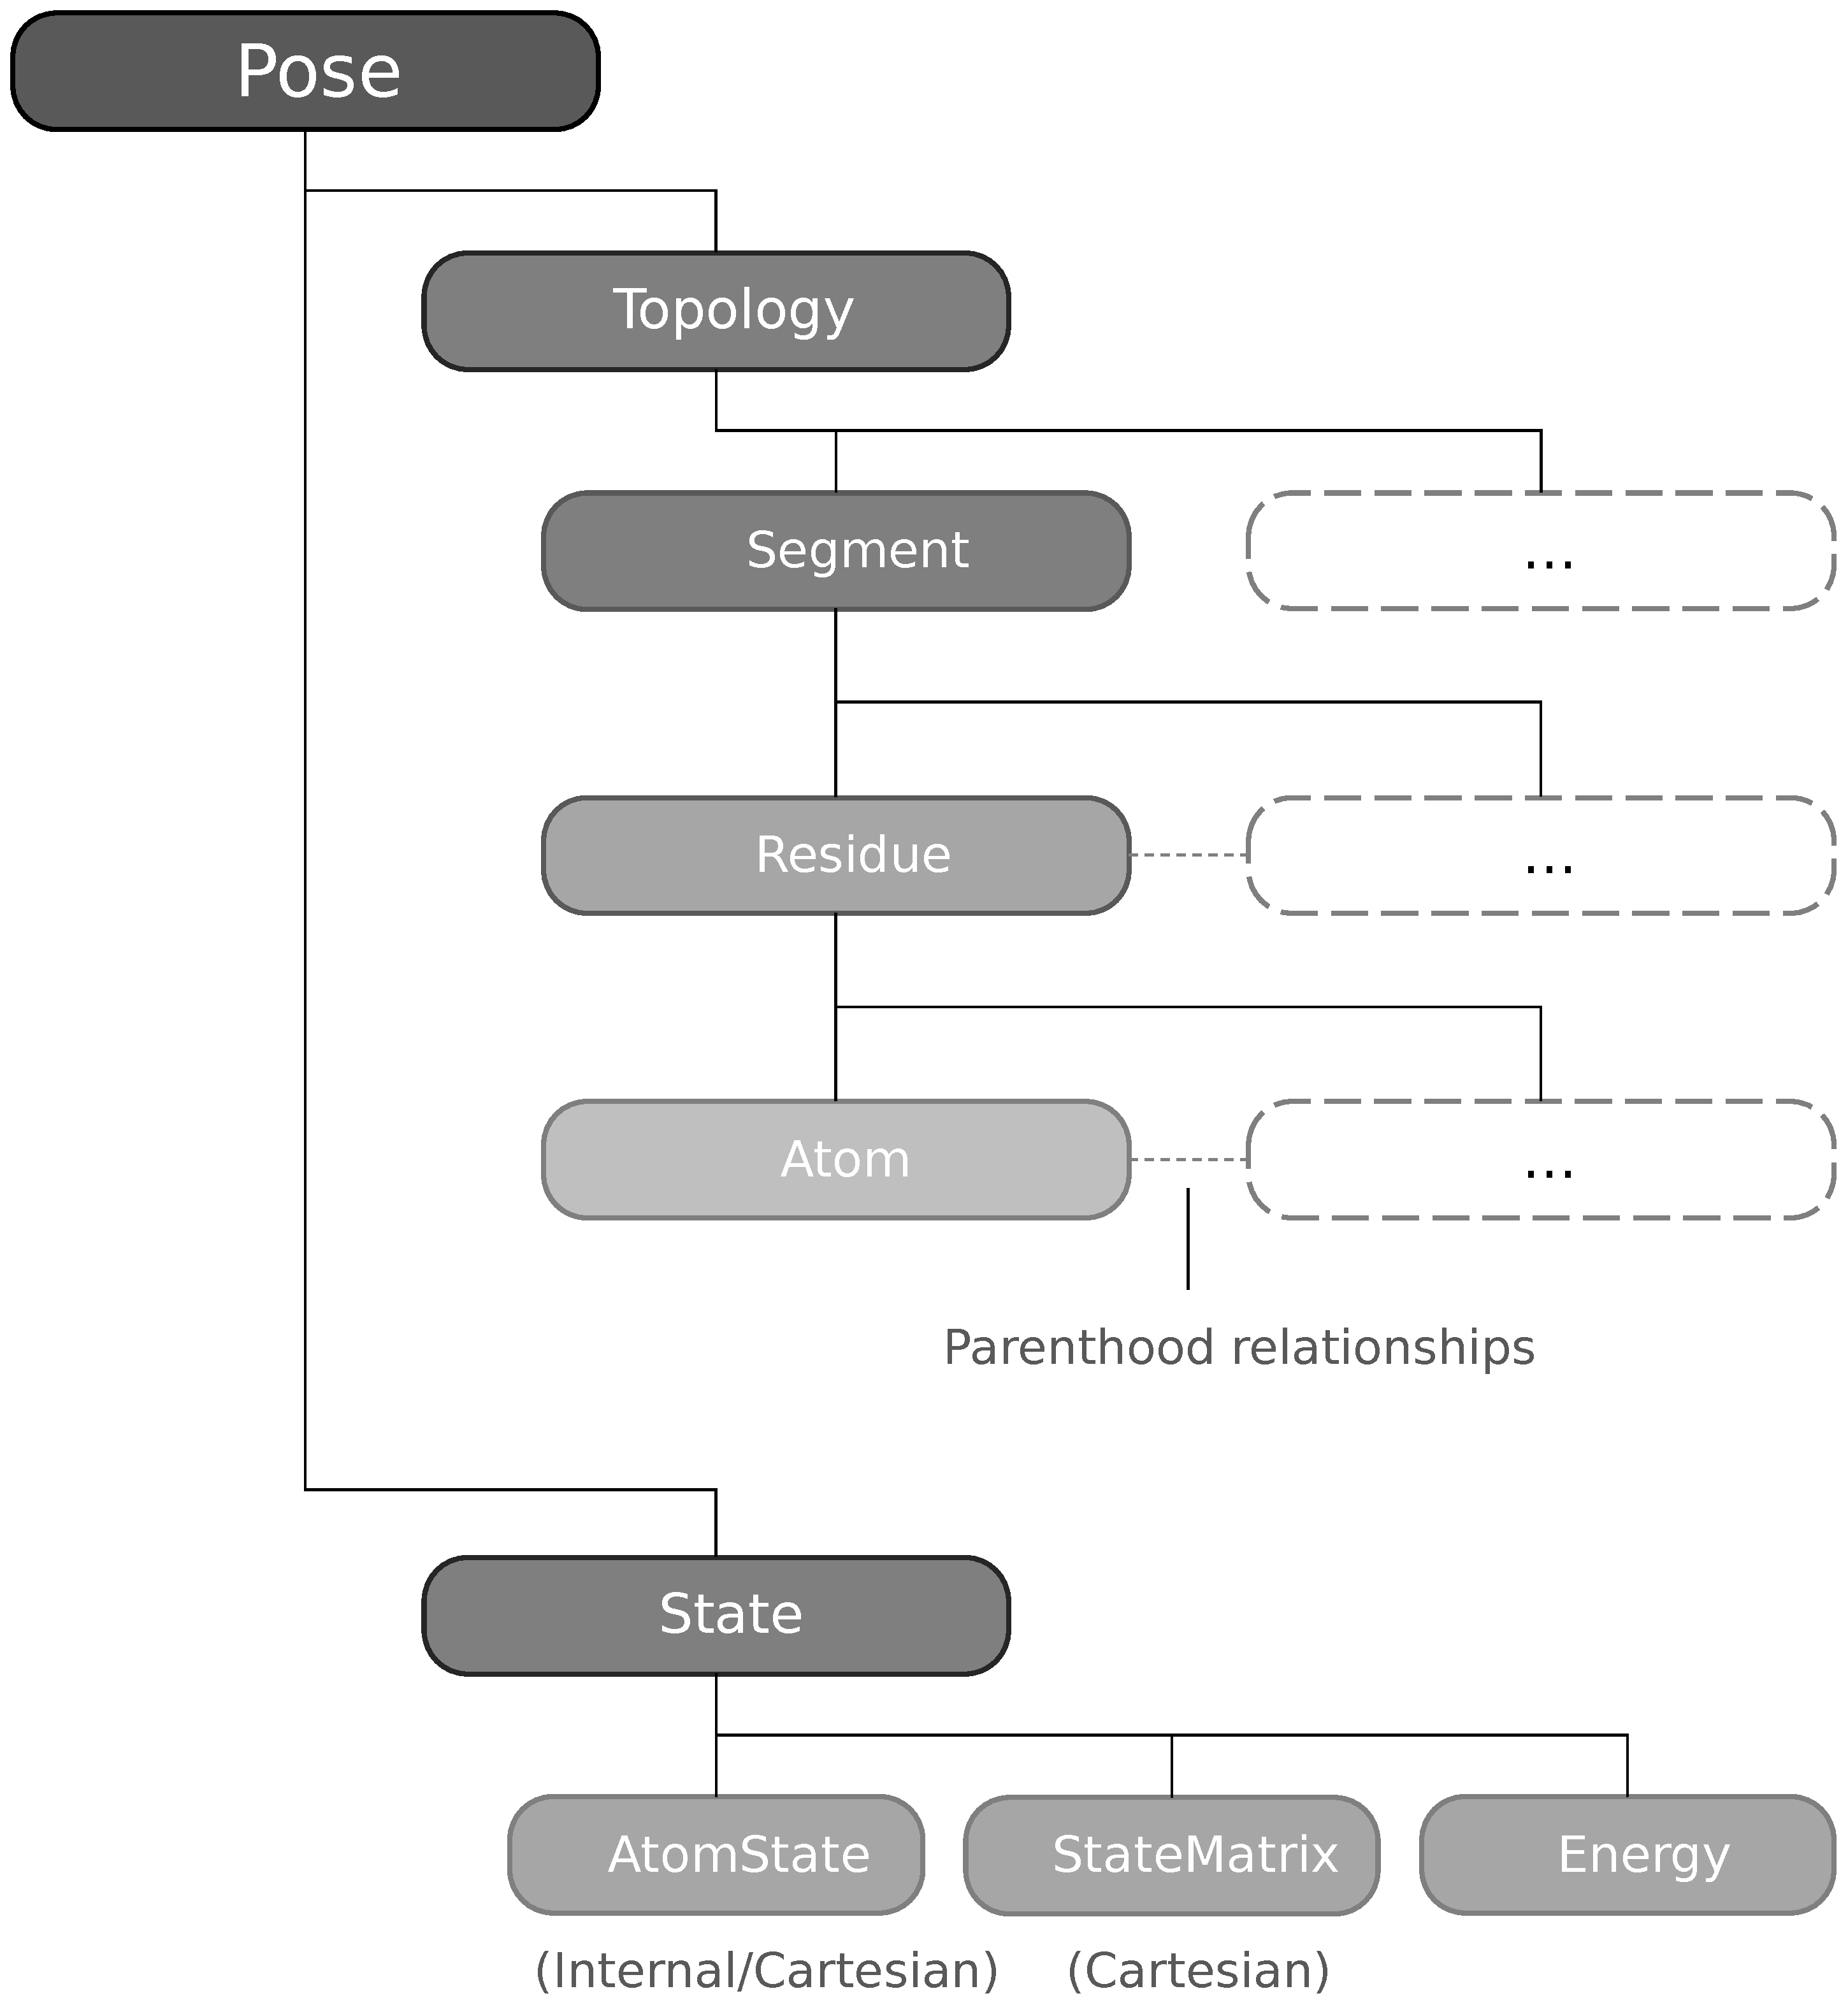
\includegraphics[width=0.45\textwidth]{ProtoSynArticle-IM2}
\caption{\textbf{ProtoSyn.jl's main structure class, the Pose.} A Pose is described by both a directed graph (under the class Topology) and a State. The Topology holds meta information regarding the nature and relationships between particles in a system, being hierarchically comprised of Segment, Residue and Atom instances. Both Residue and Atom instances have parenthood relationships between themselves. The State holds information regarding the position of the atoms both in internal and cartesian coordinates, as well as the current system’s energy.}
\label{fig:ProtoSynArticle-IM2}
\end{figure}

Firstly, the directed Graph introduces the hierarchical organization of a system: Atoms are grouped in Residues, which in turn are organized in Segments, which, finally, collectively form a Topology. Secondly, the directed Graph, as the name implies, introduces the concept of parenthood between particles in the system: each atom has a parent, and may have one or more child atoms. The same concept is extended to Residues. Ultimately, the initial atom in a Pose is a child of the Root structure, a group of three virtual atoms.\vspace{5mm}
This organization becomes particularly interesting when coupled with the State hybrid coordinate system: each system of atoms is described both by the cartesian coordinates (where each position is defined by the X, Y and Z coordinates in 3D space), as well as by the internal coordinates (in which case each position is defined by the distance, angle and dihedral angle to the parent/ascendents particles). Both coordinate systems are interchangeable and synched during simulation: in certain methods, such as a dihedral rotation, internal coordinates are both easier to use and faster to calculate, while in others, such as a rigid body movement, cartesian coordinates take precedence.\vspace{5mm}
Besides the atomic positions, a Pose’s State also holds information regarding the atomic partial charges (when necessary) and the current system’s energy.\vspace{5mm}
Most of ProtoSyn.jl’s molecular manipulation methods (such as any function implied in a mutation or in building a peptide from a sequence) make use of a stochastic L-system formal grammar \cite{Prusinkiewicz1990}: the Residues in ProtoSyn.jl are included in a grammar and can be combined from strings by a collection of production rules and an initial axiom. In the case of peptides, the production rule is linear (the peptide bond). However, the usage of this paradigm opens the path to the incorporation of randomly generated ramified carbohydrates and glycoproteins (with $\alpha$-1-4 and $\alpha$-1-6 bonds, for example), as well as allowing the incorporation of new amino acids in the available grammar, even with multiple connections between Residue instances (as is the case in some non-canonical amino acids). Besides allowing the incorporation of newly defined NCAA instances by the user, the overall architecture of ProtoSyn.jl also allows for easy introduction of modifications to existing amino acids, such as in phosphorylation and methylation post-translational processes, a recent avenue of research that has gained traction in the last few years \cite{Gang2021, Nagata2014}.\vspace{5mm}
Another interesting implication of employing L-grammars as the basis of ProtoSyn.jl is that, for most applications, atom types are replaced by a template-based approach. For example, each amino acid template includes all the required information about each individual atom, such as the default partial charge, among others, instead of requiring a costly atom typing process. In other words, the atom typing problem is replaced by an atom naming problem: for correct retrieval of information from templates, it must be possible to have a one-to-one relationship between a structure and a template. In some cases, such as when working with proteins, atom names (in this case, in the context of amino acids) are extensively conventionalized, with specific nomenclatures accepted and widely employed. Therefore, this one-to-one relationship, via the correct atom name attribution, becomes quite easy and already established in most cases.\vspace{5mm}
The above-mentioned types and methods define most of the Core module of ProtoSyn.jl: any function defined here is agnostic to the molecule type being used. Taking advantage of the multiple dispatch paradigm employed by the Julia programming language \cite{Zappa2018}, methods are extended in particular modules (such as the Peptides module), introducing specific functions that assume the molecules being simulated are of a given nature (for example, methods in the Peptides module might assume the input Pose has CA atoms). Each of these modules is usually subdivided in the following sub-modules, as schematically illustrated in Figure \ref{fig:ProtoSynArticle-IM3}:

\begin{figure}[h]
\centering
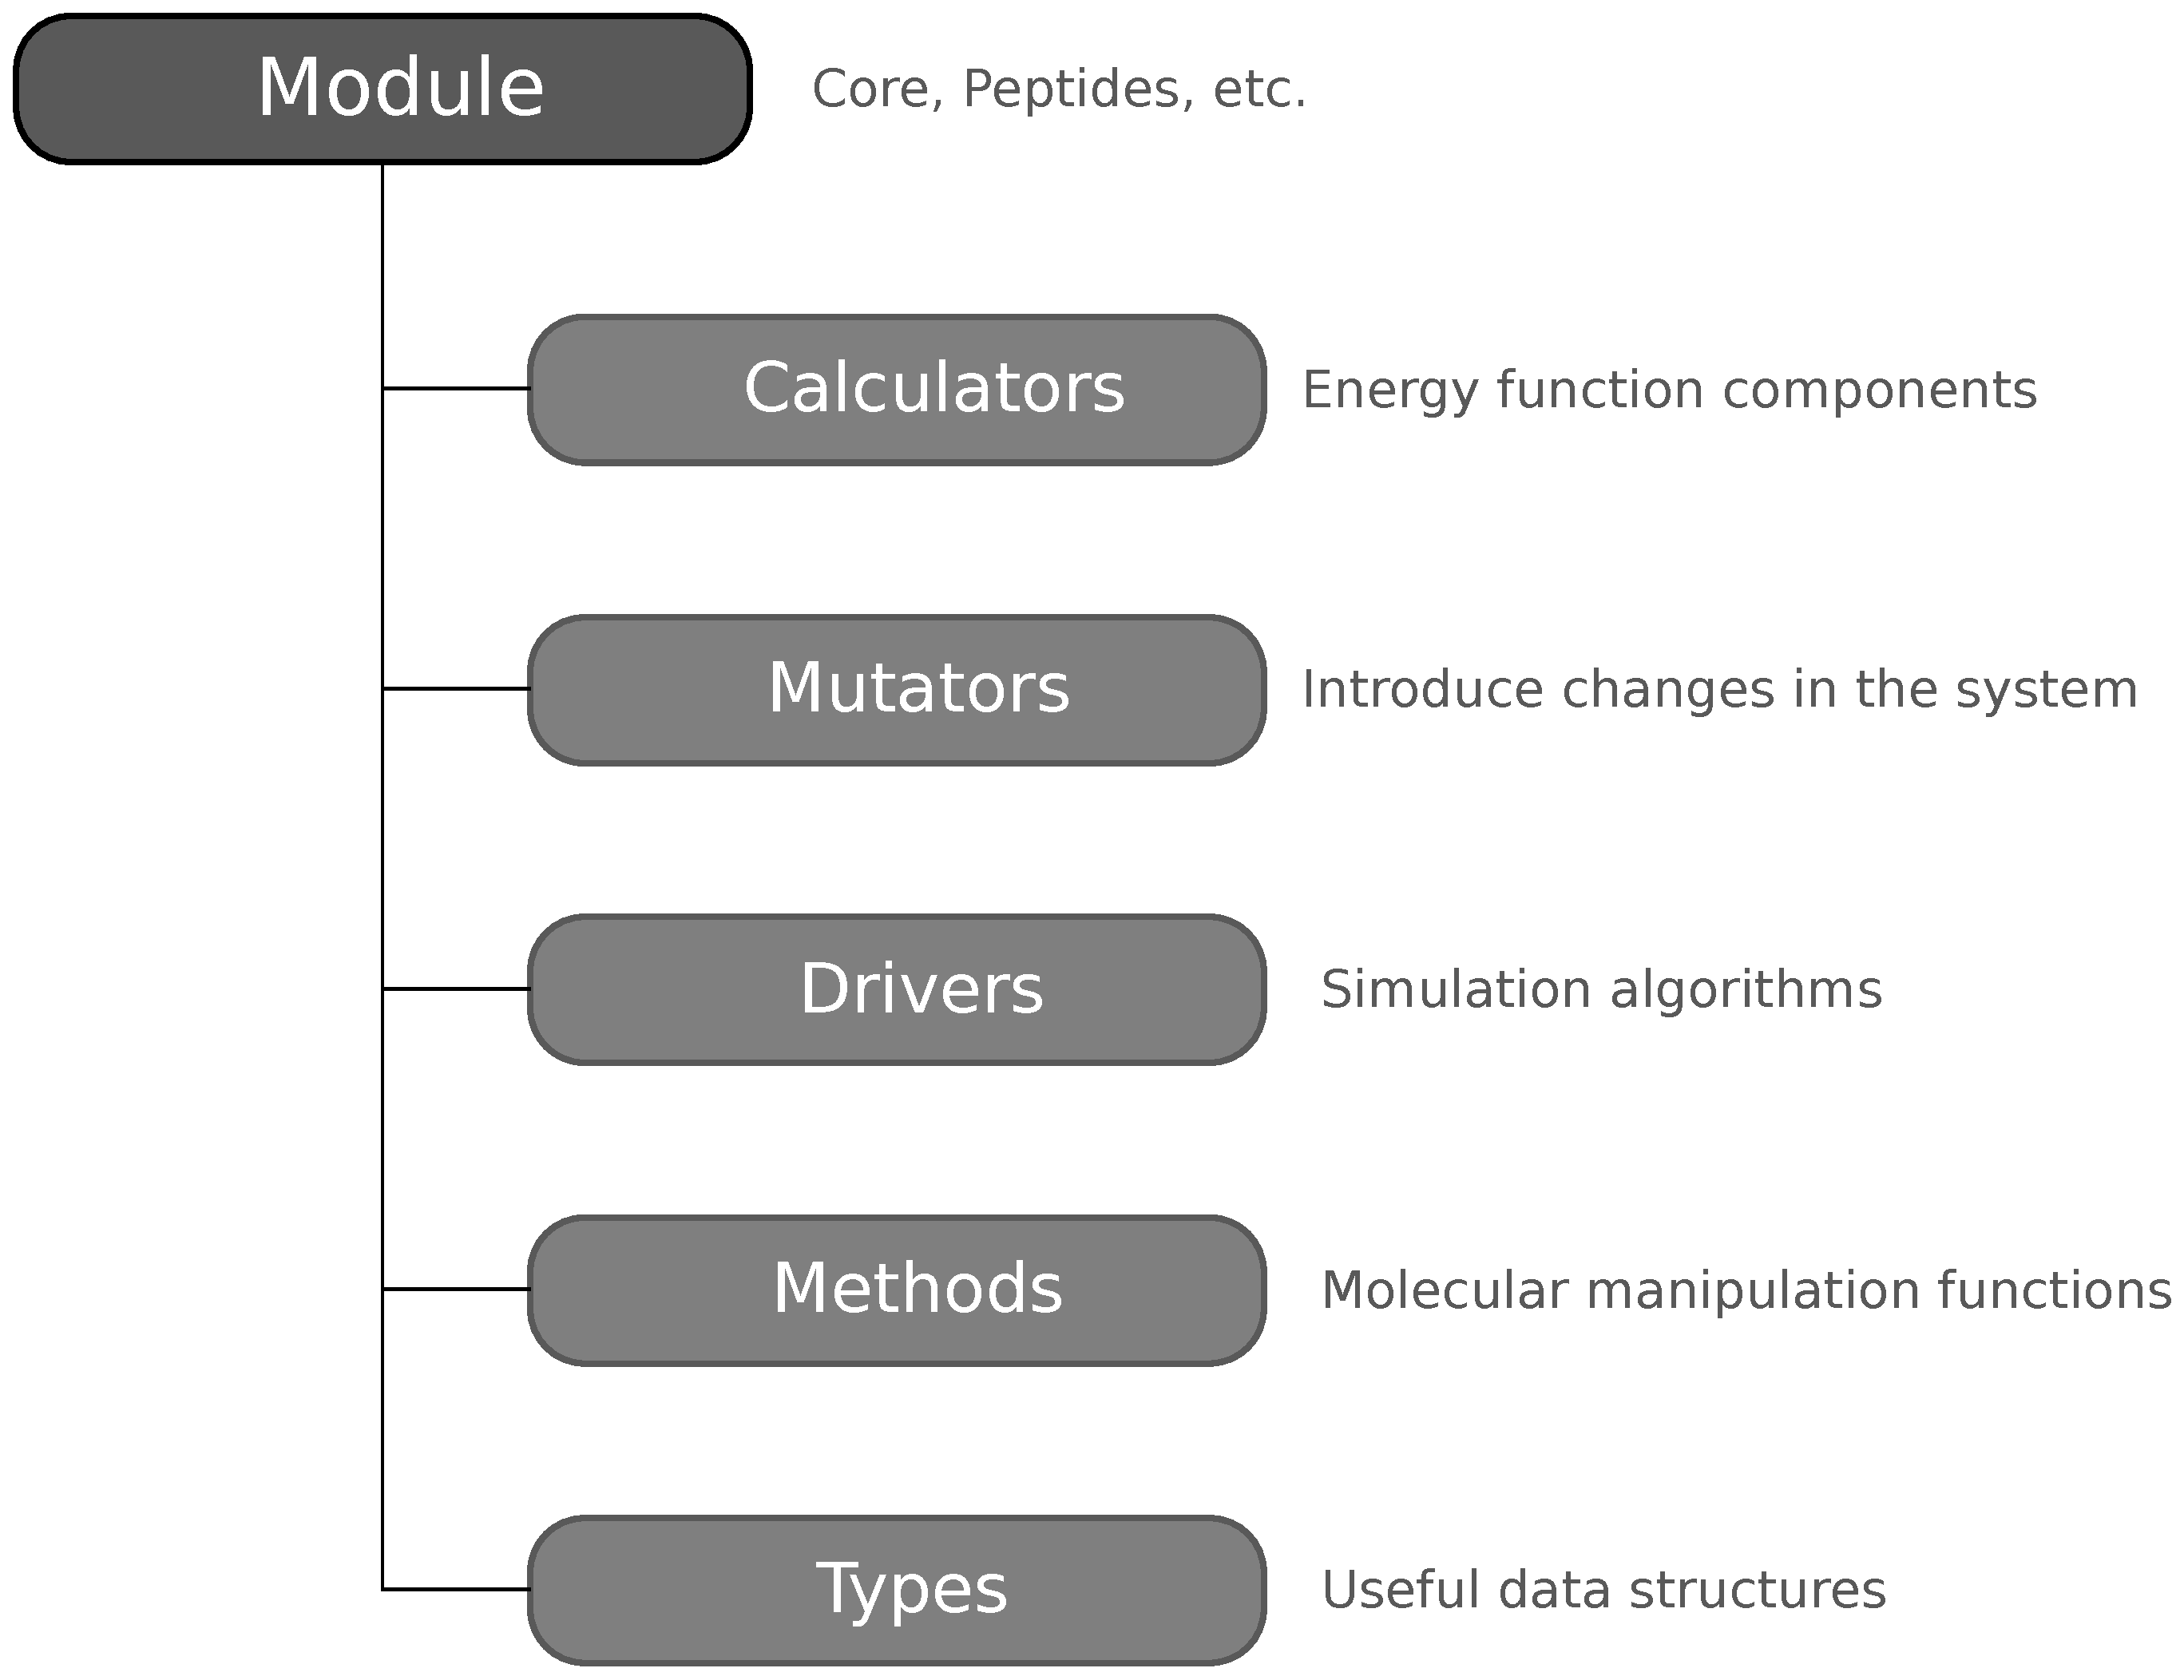
\includegraphics[width=0.45\textwidth]{ProtoSynArticle-IM3}
\caption{\textbf{ProtoSyn.jl’s modules organization.} ProtoSyn.jl’s code is organized in multiple modules, based on the target’s molecule type. The Core module is agnostic and supplies basic functions. Specialty modules (such as the Peptides module) define Calculators, Mutators and Drivers specific for a molecule type (proteins, in this example). Calculators are individual energy function components, used to evaluate a given Pose in accordance with a specified potential; Mutators introduce individual changes in a system; and Drivers are algorithms that drive the system from a state to another, in accordance with some rule. In addition, general molecular manipulation functions and useful data structures can also be found at the Methods and Types directories, respectively.}
\label{fig:ProtoSynArticle-IM3}
\end{figure}

\section{Conclusion}

Even though ProtoSyn employs this seemingly simple architecture, given the modular nature of most components, arbitrarily complex protocols and simulations can be easily constructed. In one such example, ProtoSyn was employed to determine an approximated folding structure of a small peptide, PDB 2A3D \cite{Walsh1999}. This protocol is shared here as an illustration of the usage of ProtoSyn.jl: even the simplest of protein folding prediction problems pose a challenge to any molecular manipulation and simulation software, thus benchmarking the employed energy function and performance of the platform. For the full code (including comments), see \href{https://github.com/JosePereiraUA/ProtoSyn-use-cases}{https://github.com/JosePereiraUA/ProtoSyn-use-cases}. As shown in Figures \ref{fig:ProtoSynArticle-IM4} and \ref{fig:ProtoSynArticle-IM5}, ProtoSyn.jl is able to correctly simulate the folding patterns of a small peptide (down to C$\alpha$-C$\alpha$ RMSD of 3.93 \mbox{\normalfont\AA}), plugging in several state-of-the-art models from the literature in an extremely easy way. Using the Zhang Lab TM-score online server, the predicted structure shows a TM-score of 0.5927 (excluding the sidechains). Overall, the distributed simulations, despite running for 1 million steps each, concluded in a reasonable amount of time, taking less than 120 hours to complete all 1000 replicas. As such, the distributed computing set up run an average of 2300 conformational samplings per second. Figure \ref{fig:ProtoSynArticle-IM6} showcases ProtoSyn.jl usage in high-resolution side chain clash solving.\vspace{5mm}

\begin{figure}[h]
\centering
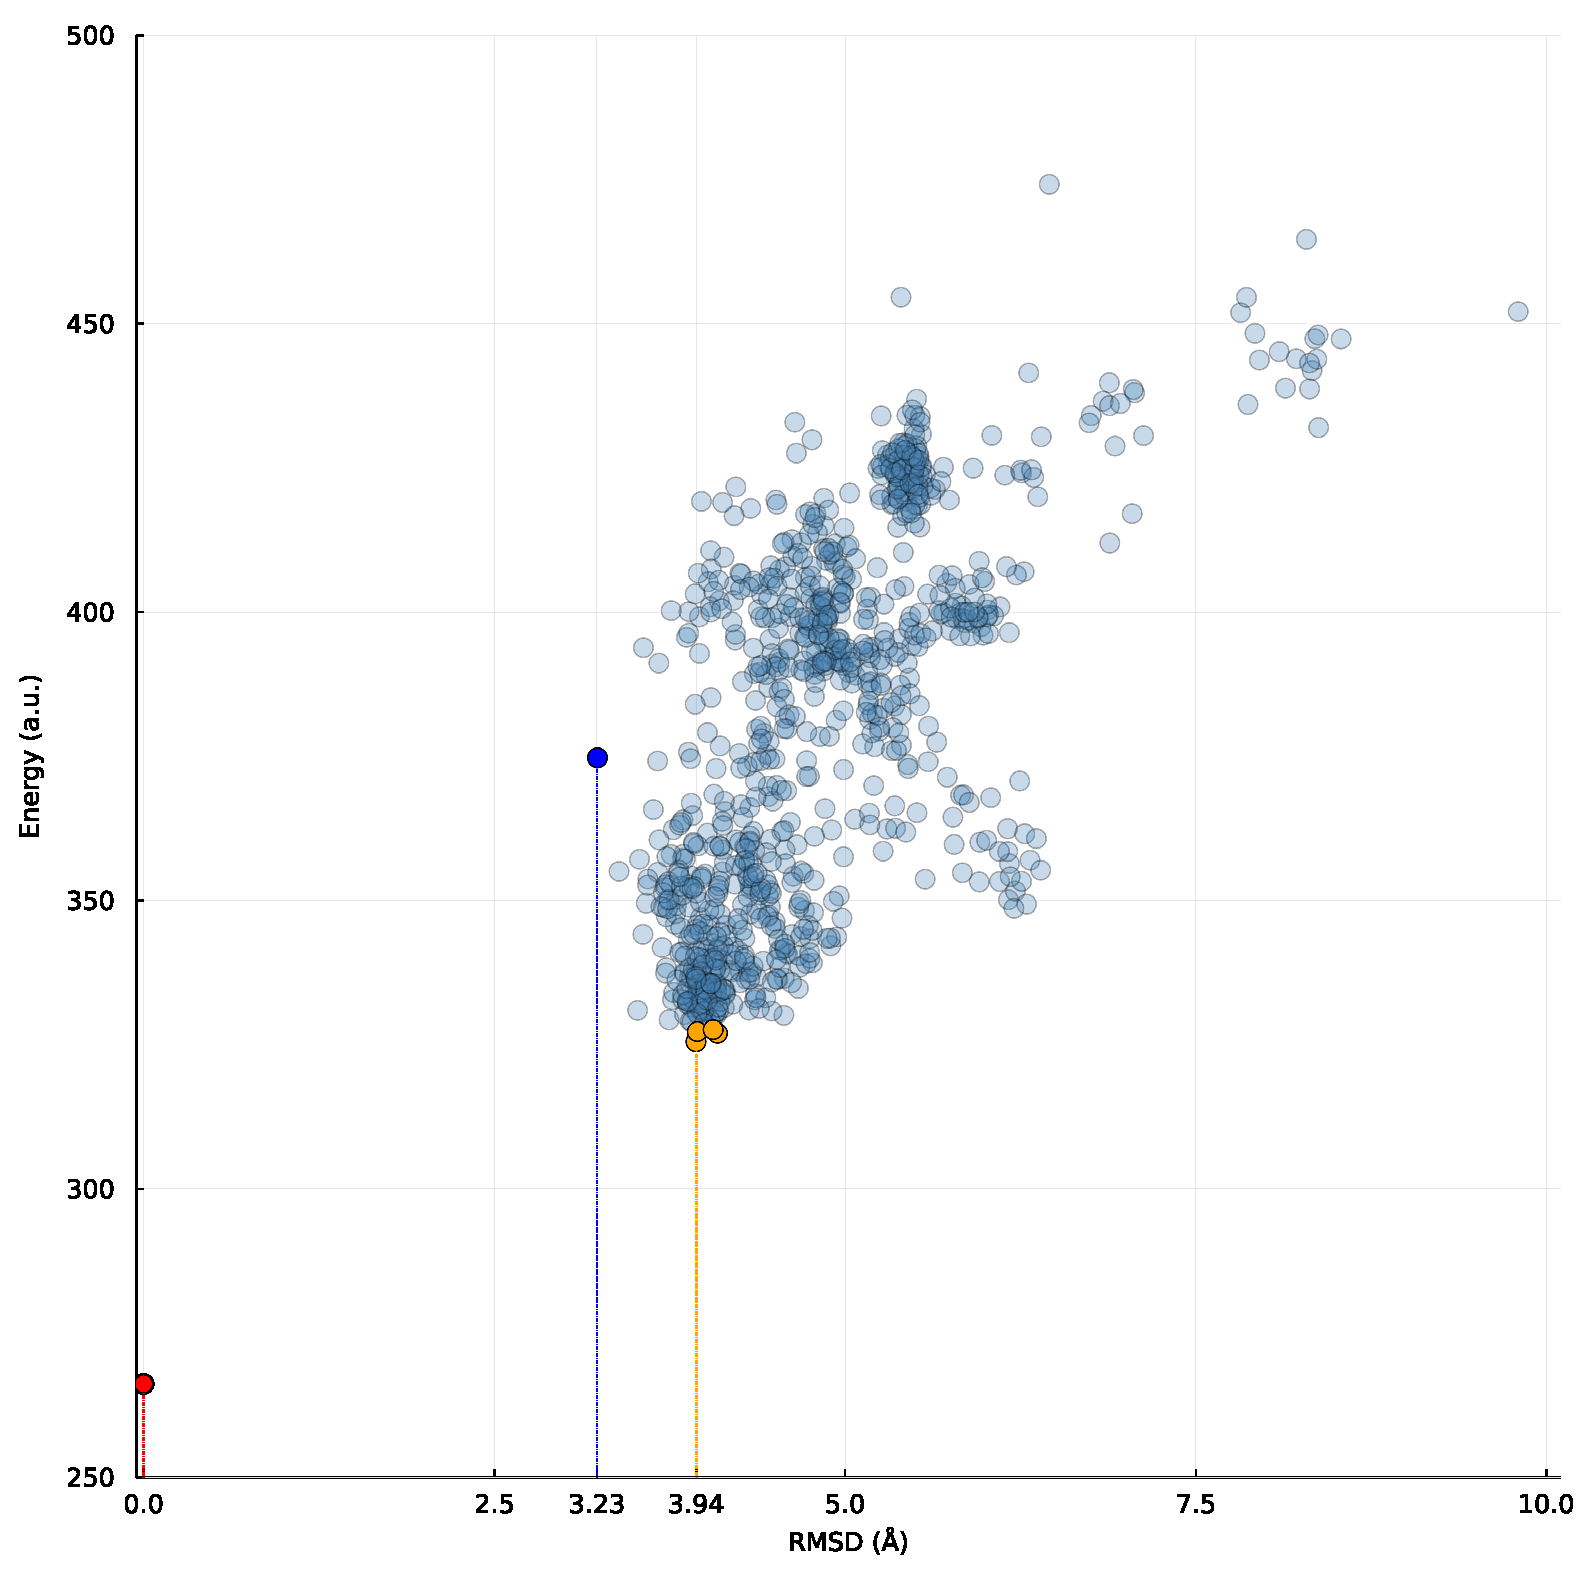
\includegraphics[width=0.45\textwidth]{ProtoSynArticle-IM4}
\caption{\textbf{Low-resolution folding prediction using ProtoSyn.jl.} In light blue, all 1000 replicas show a good folding funnel. Highlighted in yellow, the 5 lowest energy structures. Within this set, the lowest energy structure (identified by the low-resolution algorithm) showcases 3.93 Å in RMSD. Marked in dark blue, the lowest RMSD structure (not identified by ProtoSyn.jl as a low-energy structure) shows a 3.23 Å RMSD. The base truth (i. e.: the crystallographic model) is shown in red.}
\label{fig:ProtoSynArticle-IM4}
\end{figure}

\begin{figure}[h]
\centering
\includegraphics[width=0.45\textwidth]{ProtoSynArticle-IM5}
\caption{\textbf{Lowest energy candidate.} In yellow, the lowest energy Pose from the low-resolution simulation shows a 3.93 Å RMSD value when compared with the crystalline structure of the 2A3D peptide, in red.}
\label{fig:ProtoSynArticle-IM5}
\end{figure}

\begin{figure}[h]
\centering
\includegraphics[width=0.45\textwidth]{ProtoSynArticle-IM6}
\caption{\textbf{Solving sidechain clashes.} In yellow, the lowest energy Pose from the low-resolution simulation is minimized (in a high-resolution simulation) to solve atomic clashes (marked by a red arrow). A – The initial sidechain recovery is agnostic to its surroundings, often inducing atomic clashes when placing sidechains. B – After a few steps of a Monte-Carlo simulation, initial clashes are solved and the minimized structure shows a lower all-atom RMSD value.}
\label{fig:ProtoSynArticle-IM6}
\end{figure}

ProtoSyn.jl’s development constitutes a first attempt at a Julia-based molecular manipulation and simulation software. In conclusion, ProtoSyn.jl does not intend to re-invent the wheel: previous software solutions for molecular manipulation and simulation have proven, time and time again, their accuracy and performance, forever changing the landscape of how protein design is pursued. Technology development, however, is continuously adding new and better ways to do stuff and, as such, ProtoSyn.jl intends to introduce much needed quality-of-life improvements while lowering the entry barrier to non-expert users. Furthermore, it is the developer’s view that a modern scientific software’s potential is only truly unlocked by allowing and encouraging input from various sources and scientific backgrounds, in an open-source setting, while maintaining and curating a complete, correct and exhaustive documentation and examples suite. Given the implementation within the Julia environment, further interface development with emerging packages, such as Molly.jl, DTFK.jl and AtomsBase.jl will further strengthen the available suite of tools available for computational chemists interested in exploring protein design within the Julia ecosystem.

\input{bib.tex}

\end{document}

% Inspired by the International Journal of Computer Applications template
